\begin{figure}[t]
	\centering
	%\includegraphics[width=\columnwidth]{Atom-ogMolekylefysik/billeder/HX-kogepunkt.png}
	\includegraphics[width=.8\columnwidth]{HX-kogepunkt.png}
	\caption{Kogepunkterne for hydrogenhaliderne.} %Kilde: DIC.}
	\label{fig:HX-kogepunkt}
\end{figure}
\begin{opgave}{Halogener og hydrogenbindinger}{3}
Et vigtigt resultat, der lægger grunden for en masse kemi, er at elektronkonfigurationer, hvor den yderste $s$- og $p$-orbital er fyldte, er særligt stabile, hvilket leder til hvad der i kemi kaldes "oktetreglen". Dette resultat har nogle interessante konsekvenser, der her vil undersøges.
\opg Hvilken elektronkonfiguration har flour, $F$, der er grundstof nummer 9?
\opg Flour står i 17. gruppe, der også kaldes halogenerne, som alle er karakteriseret ved at have samme elektronkonfiguration i deres yderste $s$- og $p$-orbitaler. Hvorfor er denne konfiguration speciel?
\opg Ligesom hydrogen samler halogenerne sig i molekyler på formen $\mathrm{X}_2$, hvor X er et vilkårlig halogen. Blandes en halogengas med hydrogengas forekommer følgende reaktion
\begin{align*}
	\mathrm{H}_2(g) + \mathrm{X}_2(g) \rightarrow 2 \mathrm{HX}(g)
\end{align*}
Forklar med et molekylorbitaldiagram, hvorfor HF er mere stabilt end $\mathrm{H}_2$ og $\mathrm{F}_2$.
\opg Hvilke atomorbitaler danner bindingen i HF og hvilken type er det?
\opg I eksemplet med $\mathrm{H}_2$ er de to atomer ens, hvorfor orbitalen er symmetrisk omkring en akse midt imellem de to atomer. Hvis de to atomer er forskellige, eller det ikke er samme orbitaler der binder, er dette ikke nødvendigvis sandt. Hvorfor er molekylorbitalen for HF forskudt og imod hvilket atom?
\opg Denne forskydning giver HF et dipolmoment\footnote{Mere præcist kan det siges at der er størst sandsynlighed for at de bindende elektroner befinder sig tættere på F end H, og ikke omvendt eller ligeligt fordelt. Det betyder at forventningsværdien, $\expect{\v{r}}$, vil være forskudt mod flour. Det siges derfor ladningen i gennemsnit samler sig hos flour, som så er partielt negativt ladet, mens H er partielt positivt ladet.}, hvilket i denne sammenhæng fint kan tænkes som en ladningsforskydning, hvor alle elektronerne befinder sig tættere på F end H. Forklar hvorfor det betyder at molekylerne tiltrækkes af hinanden, hvilket kaldes hydrogenbindinger?
\opg HF er det eneste af hydrogenhaliderne, HX, der kan danne hydrogenbindinger, hvilket kan ses på deres kogepunkter, figur \ref{fig:HX-kogepunkt}. Hvorfor det? \\
Netop denne forskel gør flussyre, der er en vandig opløsning af HF, speciel. Den er i modsætning til de andre hydrogenhalider i stand til at opløse glas, hvorfor den ikke er så let at opbevare. Derudover kan den trænge igennem huden og opløse kroppen indefra, hvorfor eksempelvis saltsyre, HCl, oftere benyttes.
\end{opgave}